\section{Image Denoising} % (fold)
\label{sec:image_denoising}
    
    Denoising images is a hard task. As discussed before, an image $g$ consists of data and noisy. Our goal is to remove the noise from an input image $g$ and get a smooth approximation $u$. We find different kinds of noise on images. The two most common are Gaussian noise and the so called salt and pepper noise. Where Gaussian noise is relatively easy to remove, salt and pepper noise is more robust since it resembles extrem values on images. 
% section image_denoising (end)

\begin{figure}[ht]
    \centering
    \begin{subfigure}[b]{0.45\textwidth}
        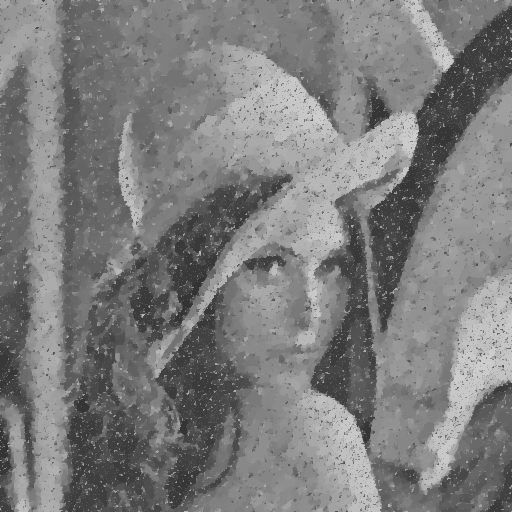
\includegraphics[width=\textwidth]{img/denoising/gauss_noise/rof/002lena.png}
        \caption{$\lambda = 0.02$}
    \end{subfigure}
    \begin{subfigure}[b]{0.45\textwidth}
        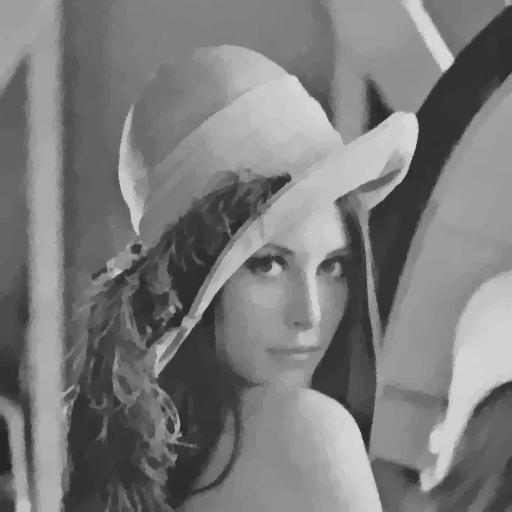
\includegraphics[width=\textwidth]{img/denoising/gauss_noise/rof/003lena.png}
        \caption{$\lambda = 0.03$}
    \end{subfigure}
    \caption{Denoising of Salt and Pepper noise of the Lena image with the ROF Model.}
\label{fig:denoising_lena_rof_gauss}
\end{figure}

\begin{figure}[ht]
    \centering
    \begin{subfigure}[b]{0.45\textwidth}
        \includegraphics[width=\textwidth]{img/denoising/gauss_noise/tvl1/05lena.png}
        \caption{$\lambda = 0.5$}
    \end{subfigure}
    \begin{subfigure}[b]{0.45\textwidth}
        \includegraphics[width=\textwidth]{img/denoising/gauss_noise/tvl1/06lena.png}
        \caption{$\lambda = 0.6$}
    \end{subfigure}
    \begin{subfigure}[b]{0.45\textwidth}
        \includegraphics[width=\textwidth]{img/denoising/gauss_noise/tvl1/07lena.png}
        \caption{$\lambda = 0.7$}
    \end{subfigure}
    \begin{subfigure}[b]{0.45\textwidth}
        \includegraphics[width=\textwidth]{img/denoising/gauss_noise/tvl1/08lena.png}
        \caption{$\lambda = 0.8$}
    \end{subfigure}
    \caption{Denoising of Gaussian noise of the Lena image with the TVL1 Model.}
\label{fig:denoising_lena_tvl1_gauss}
\end{figure}

\begin{figure}[ht]
    \centering
    \begin{subfigure}[b]{0.45\textwidth}
        \includegraphics[width=\textwidth]{img/denoising/salt_and_pepper_noise/rof/0007lena.png}
        \caption{$\lambda = 0.007$}
    \end{subfigure}
    \begin{subfigure}[b]{0.45\textwidth}
        \includegraphics[width=\textwidth]{img/denoising/salt_and_pepper_noise/rof/0008lena.png}
        \caption{$\lambda = 0.008$}
    \end{subfigure}
    \caption{Denoising of Salt and Pepper noise of the Lena image with the ROF Model.}
\label{fig:denoising_lena_rof_sap}
\end{figure}

\begin{figure}[ht]
    \centering
    \begin{subfigure}[b]{0.45\textwidth}
        \includegraphics[width=\textwidth]{img/denoising/salt_and_pepper_noise/tvl1/05lena.png}
        \caption{$\lambda = 0.5$}
    \end{subfigure}
    \begin{subfigure}[b]{0.45\textwidth}
        \includegraphics[width=\textwidth]{img/denoising/salt_and_pepper_noise/tvl1/06lena.png}
        \caption{$\lambda = 0.6$}
    \end{subfigure}
    \begin{subfigure}[b]{0.45\textwidth}
        \includegraphics[width=\textwidth]{img/denoising/salt_and_pepper_noise/tvl1/07lena.png}
        \caption{$\lambda = 0.7$}
    \end{subfigure}
    \begin{subfigure}[b]{0.45\textwidth}
        \includegraphics[width=\textwidth]{img/denoising/salt_and_pepper_noise/tvl1/08lena.png}
        \caption{$\lambda = 0.8$}
    \end{subfigure}
    \caption{Denoising of Salt and Pepper noise of the Lena image with the TVL1 Model.}
\label{fig:denoising_lena_tvl1_sap}
\end{figure}